A migratory typing system adds static types onto a
dynamically-typed host language.
At a minimum, the addition requires a static type checker and an extended
syntax to accomodate mixed-typed code.
If the types are intended to serve as claims about the kinds of values that
flow through a program at run-time, then the addition also requires a method
of enforcing types.

Typed Racket~\cite{tf-popl-2008} is one example of a migratory typing system; it adds
a new language, \racketcode{\#lang typed/racket}, to Racket.
The language accepts type-annotated Racket programs,
validates the annotations with a sophisticated type checker~\cite{tf-icfp-2010},
and enforces the annotations with higher-order contracts.
For example, \figureref{fig:guess-game} presents a mixed-typed
program consisting of three modules.
The two untyped modules at the top of the figure define a guessing game
and a game player.
The typed module at the bottom gives the player five chances to submit a
correct guess.

Technically, both the guessing game and the player are represented as functions.
The typed driver module assigns a static type to each function.
At compile-time, the type checker validates the contents of the driver module
\emph{assuming}\/ that the types assigned to the untyped functions are correct.
At run-time, higher-order contracts dynamically enforce the claims in the types.
Thanks to the contracts, these types are kept honest.

\begin{figure}[h]
  \begin{minipage}[t]{0.45\columnwidth}
    \begin{lstlisting}
#lang racket
(provide play)

(define (play)
  (define n (random 10))
  (lambda (guess)
    (= guess n)))
    \end{lstlisting}

  \end{minipage}\begin{minipage}[t]{0.45\columnwidth}
    \begin{lstlisting}
#lang racket
(provide stubborn-player)

(define (stubborn-player i)
  4)
    \end{lstlisting}

  \end{minipage}

  \smallskip
  \begin{centering}
    \begin{minipage}{0.6\columnwidth}
      \begin{lstlisting}
#lang typed/racket

(require/typed "guess-game.rkt"
  [play (-> (-> Natural Boolean))])
(require/typed "stubborn-player.rkt"
  [stubborn-player (-> Natural Natural)])

(define check-guess (play))

(for/or ([i : Natural (in-range 5)])
  (check-guess (stubborn-player i)))
      \end{lstlisting}
    \end{minipage}
  \end{centering}

  \caption{A mixed-typed Typed Racket program~\cite{gtnffvf-jfp-2019}}
  \label{fig:guess-game}
\end{figure}

In theory, Typed Racket lets programmers freely mix typed and untyped modules.
The maintainer of a large untyped codebase may add types to any
 one module while leaving the rest untyped.
After the conversion, the new module benefits from static type checking
 and type-based compiler optimizations; the full mixed-typed codebase can
 be run without further changes.
Running the code may reveal a dynamic mismatch; in particular, an untyped value
 that flows into the newly-typed module may fail to live up to the type annotations.
If so, the program halts and the programmer can fix the types
 and/or the untyped code accordingly.
Adding types thus leads to incremental improvements.

In practice, a programmer's freedom to add types is severly limited by
 the run-time cost of type enforcement.
Adding types to one module adds a contract boundary to its neighbors.
When two modules communicate through a boundary, they may experience three kinds
 of performance overhead.
First, there is the obvious cost of checking every value that crosses the
 boundary.
Second, a higher-order boundary must allocate a new wrappers to constrain the
 future behavior of any values that cross it.
Third, wrapped values suffer from a layer of indirection.
These costs may increase the overall running time of a program by an order
 of magnitude (\figureref{fig:max-overhead}).
Clearly, keeping types honest may impose a huge cost.

\begin{figure}[h]
  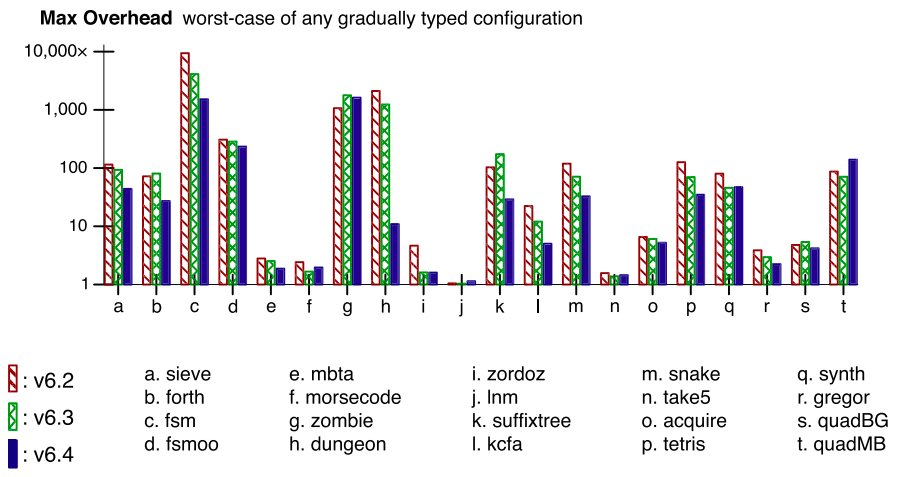
\includegraphics[width=0.8\columnwidth]{src/jfp-2019-max.png}
  \caption{Worst-case overheads across 20 benchmarks and 3 versions of Typed Racket~\cite{gtnffvf-jfp-2019}}
  \label{fig:max-overhead}
\end{figure}
%\footnote{\shorturl{https://}{docs.racket-lang.org/gtp-benchmarks/index.html}}

Other migratory typing systems take a different approach to type enforcement.
Instead of keeping types honest, they perform incomplete checks,
 provide weaker guarantees, and offer different performance tradeoffs.



During compilation, the Typed Racket type checker validates the expre

by assigning a type
annotation to each.

Technically, the guessing game is a higher-order thunk; when invoked, it
chooses a random number and returns a new procedure that compares the number
to a guess.
The game player is also a procedure.


When
When i

Turning up.

%Programs in the new language 
%
%The syntax of the new language 
%
%Typed code is validated by a stati
%
%
%It adds a new language to Racket, 
%accepts type-annotated Racket programs.
%
%
%A type checker validates the annotations
%
%The literature contains many other examples; see \citet{gf-icfp-2018} for a
%brief survey.
%
%for Racket.
%
%Typed Racket extends the syntax
%
% extends the syntax of Racket with a 
%

- - -

Ultimately, the goal is something practical.
Bring research type systems to widely-used languages.

- - -

Began with a capable implementation of migratory typing; namely, Typed Racket.
That proof-of-concept back in 2006 had matured to support all kinds of Racket programs.
It also clearly had performance troubles, identified by users around the world.

The question was, how bad is performance?
To answer, we developed a method and conducted an evaluation.
The results were quite bad, inspired a lot of improvements, and are still a challenge today.

Meanwhile, other groups explored migratory typing in other contexts.
Transient Reticulated particularly interesting.
We adapted the evaluation method to Transient.
Findings --- on completely different benchmarks --- were encouraging in a big (order of magnitude) way.

Compared Transient style to Typed Racket style on Racket programs.
Performance results confirm findings from the Transient-alone study.

Developed models to state and prove properties for each.
Different type soundness!
Whats more, different about trusting the types.
TR-style is a complete monitor but Transient-style is not.


